\section{Results}\label{sec:results}
\subsection{Static rankings: the choice matters where the model is still useful}\label{sec:static}
Figure~\ref{fig:ber} shows task quality against BER at 12.5\% protection. At low BER all masks are indistinguishable from clean operation, and at the highest BERs every mask fails. In between lies a band, one to two decades wide, where the model is useful under some masks and not under others; that band is where protection decisions have consequences. For ResNet-8 at $p=3\times10^{-3}$, accuracy is 36.8\% unprotected, 70.3\% with MSB-first, 80.9\% with the global gradient and 83.0\% with the absolute gradient, against 88.0\% clean; the paired gain of absolute gradient over MSB-first is 12.7 points (95\% interval 8.4 to 16.9). For Qwen3-0.6B at $p=3\times10^{-3}$ the NLL increase is 7.60 nats per token unprotected, 0.88 with MSB-first and 0.27 with either gradient ranking.

\begin{figure}[tbp]
\centering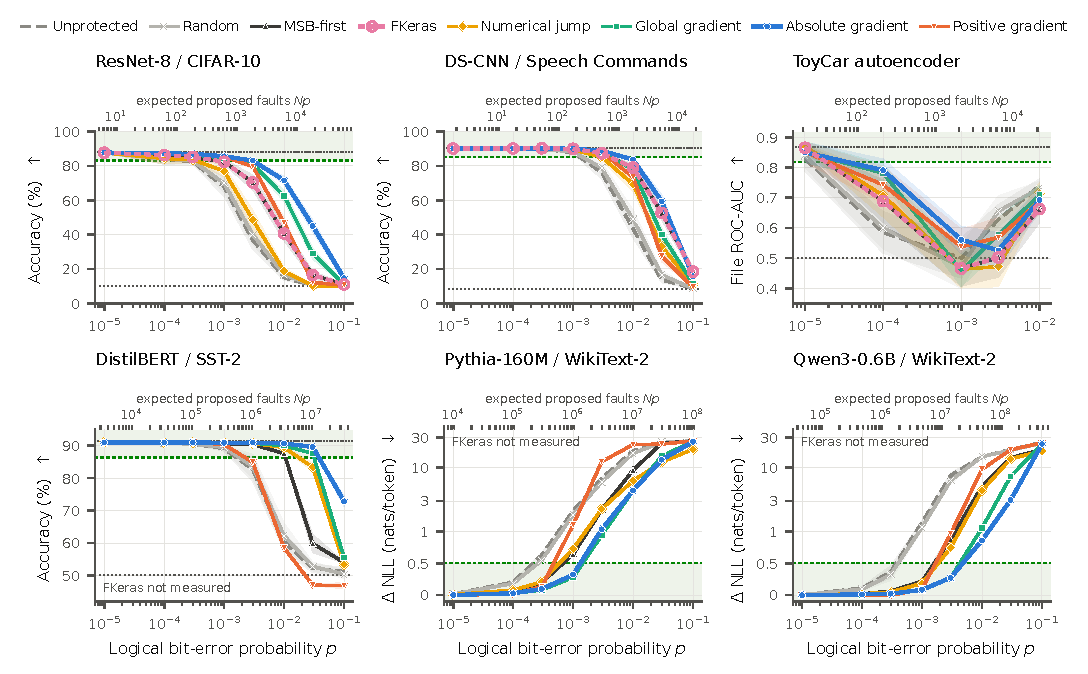
\includegraphics[width=\linewidth]{tecs_task_quality_ber_125}
\caption{Task quality versus logical BER at 12.5\% protection, with the expected number of proposed faults on the top axis. Bands are 95\% intervals of the field mean. The shaded region is the usefulness margin; dotted lines mark clean quality and chance. FKeras (open circles) was measured on the three TFLite models only; at this complete-tier budget it selects the same mask as MSB-first. Language-model panels use a symmetric-log axis.}\label{fig:ber}
\Description{Six panels of accuracy, AUC or NLL against bit-error probability for seven protection policies.}
\end{figure}

\begin{table}[t]
\caption{Highest measured BER, in units of $10^{-4}$, at which each ranking keeps mean task quality within the usefulness margin, at 12.5\% / 25\% protection. Unprotected has no budget. FKeras equals MSB-first at these two budgets.}\label{tab:useful}
\centering\small
\begin{tabular}{l r r r r r}\toprule
Ranking & ResNet-8 & DS-CNN & DistilBERT & Pythia & Qwen\\\midrule
Unprotected & 1 & 10 & 10 & 1 & 3\\
Random & 1 / 3 & 10 / 10 & 10 / 10 & 1 / 3 & 3 / 3\\
MSB-first & 3 / 10 & 30 / 100 & 100 / 100 & 3 / 10 & 10 / 30\\
Numerical jump & 3 / 3 & 10 / 30 & 100 / 300 & 3 / 10 & 10 / 30\\
Global gradient & 10 / 30 & 30 / 100 & 300 / 300 & 10 / 30 & 30 / 100\\
Absolute gradient & 30 / 30 & 30 / 100 & 300 / 1000 & 10 / 10 & 30 / 100\\
Positive gradient & 10 / 30 & 30 / 30 & 10 / 30 & 3 / 3 & 10 / 30\\\bottomrule
\end{tabular}
\Description{Highest useful bit-error probability for seven policies on five models at two budgets.}
\end{table}

Table~\ref{tab:useful} condenses the grid into the highest measured BER at which each ranking keeps the model useful. At 12.5\% protection the absolute-gradient mask extends the useful range over MSB-first by a factor of ten on ResNet-8 and three on DistilBERT, Pythia and Qwen, and over the unprotected model by three to thirty. These factors are resolved only to the half-decade grid and depend on the input window: on nine further ResNet-8 windows (Section~\ref{sec:default}) they are three and ten, while the accuracy losses at $3\times10^{-3}$ for absolute gradient, MSB-first and no protection (3.0, 16.1 and 44.5 points) agree with the original window (5.0, 17.7 and 51.2). ToyCar cannot inform the choice: its only decision-useful cells are the four at $p=10^{-5}$, where the unprotected model is itself useful (Appendix~\ref{app:evidence}).


Appendix~\ref{app:static} gives the detailed static-ranking results. With masks from 64 calibration inputs, the absolute-gradient mask keeps its largest regret below 0.7 accuracy points across new calibration draws, input windows, pruned checkpoints and retrained copies of ResNet-8, and no search-based or literature-derived allocator beats it by a point where the model is usable (Appendix~\ref{app:search}). Significance-first protection loses 9 to 34 points to it on every ResNet-8 checkpoint at $p=3\times10^{-3}$. The positive-gradient mask, which keeps the sign of a flip's effect, behaves as Section~\ref{sec:theory} predicts: on the language models it is best at the lowest rates and worst at moderate ones, on DistilBERT and Pythia it is worse than no protection in several cells, and on the under-trained ResNet-8 it lifts accuracy above the clean model at $p=10^{-3}$ and loses 22.6 points at $10^{-2}$. With 1,024 calibration inputs the same reversal appears on all nine ResNet-8 checkpoints: the positive-gradient mask is ahead in every usable cell at $10^{-3}$ and behind in every usable cell at $10^{-2}$, with resolved wins in both directions on five checkpoints (Appendix~\ref{app:calibration}). The rest of this section tests whether the theory predicts these switches and whether an assignment built from it avoids them.

\subsection{Predicting where the preferred ranking switches}\label{sec:switch}
\begin{figure}[t]
\centering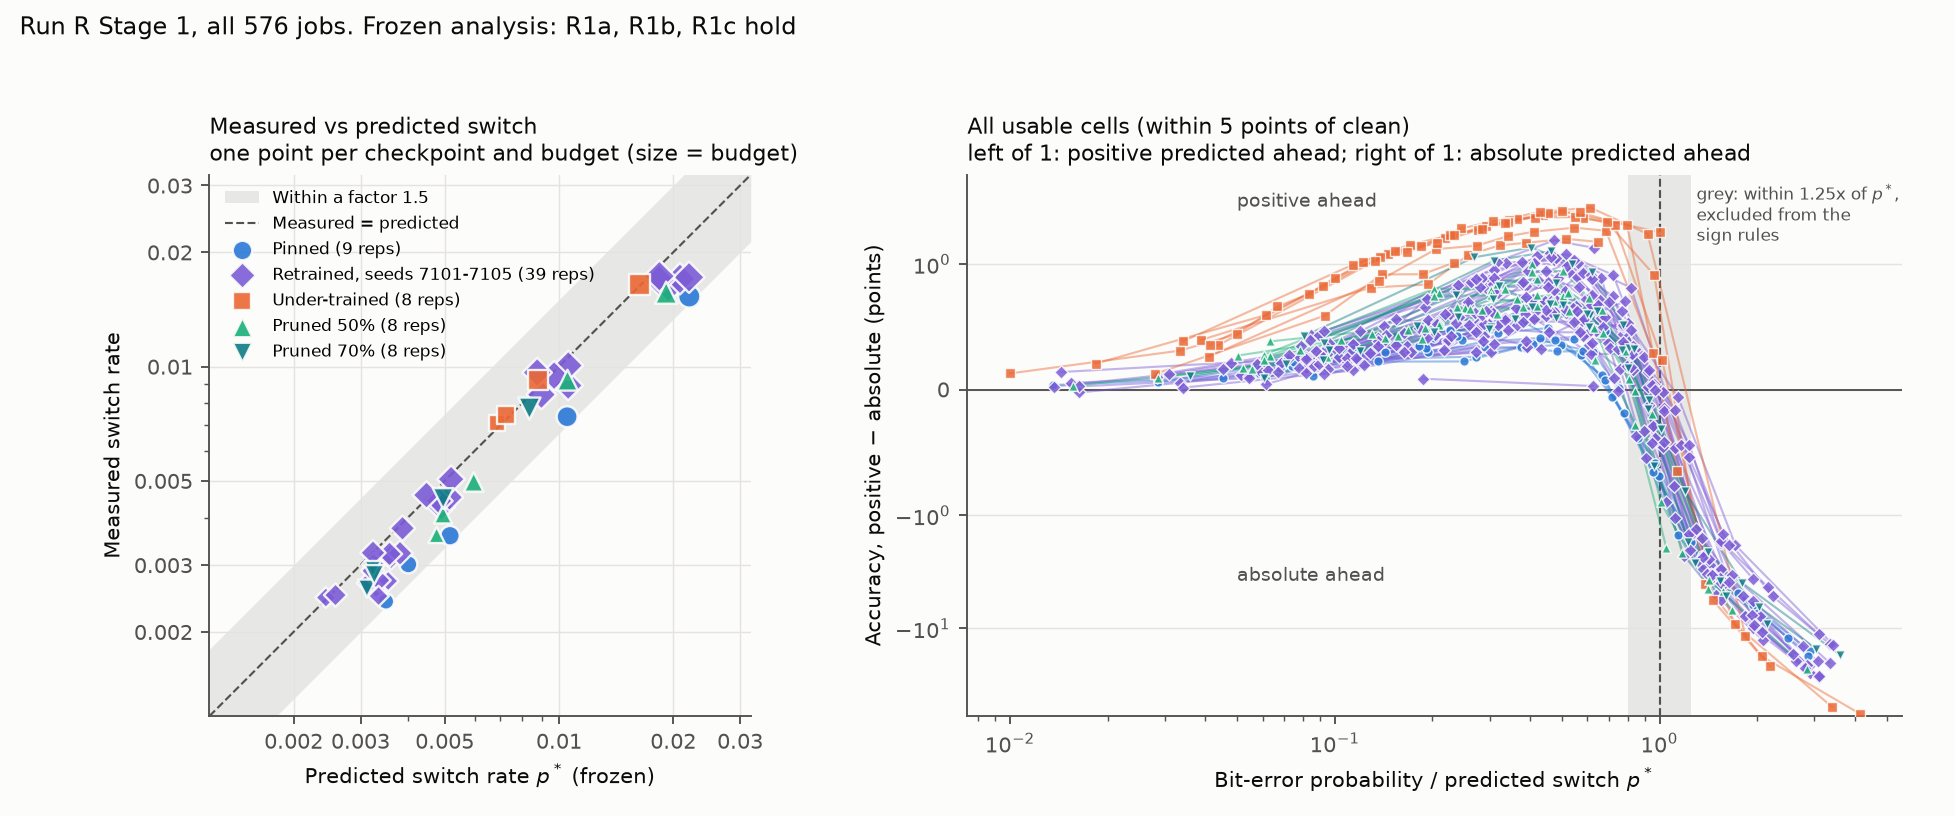
\includegraphics[width=\textwidth]{figures/stage1_switch.png}
\caption{Predicted and measured switch between the positive- and absolute-gradient masks on nine ResNet-8 checkpoints. Left: measured against predicted switch rate, one point per checkpoint and budget, with the factor-1.5 band fixed in advance. Right: accuracy of the positive minus the absolute mask in every usable cell, against the bit-error probability divided by its predicted switch; all curves cross zero near 1. The predicted switch is computed from 512 held-out training images without fault injection and was frozen before the fault fields were drawn.}\label{fig:switch}
\Description{Measured accuracy difference between two gradient masks against bit-error probability, with the predicted switch rate.}
\end{figure}
Figure~\ref{fig:switch} compares the predicted switch with the measurement on fresh fault fields. \Branch{R1}{The sign of the measured difference agrees with the prediction in 515 of the 519 usable cells away from the switch, and in all 404 of them that are resolved after Holm correction; the four exceptions are below 0.2 points. The measured switch is 0.88 times the predicted one (95\% interval over the nine checkpoints 0.80 to 0.96), within the factor of 1.5 fixed in advance. It moves with the budget as predicted, from about $2.6\times10^{-3}$ at 6.25\% to about $1.5\times10^{-2}$ at 50\% (geometric means over checkpoints), and it is highest on the under-trained checkpoint, the one farthest from a minimum ($9.5\times10^{-3}$ against $4.8$ to $5.8\times10^{-3}$ for the well-trained ones). Below 6.25\% the network loses more than 5 points before the masks swap order, so no switch is measured there.}{\TBD{Which of R1a, R1b and R1c failed, and by how much.} The prediction \TBD{e.g., gets the sign right but places the switch \ldots}.} The formula places the switch about 12\% late on average (geometric mean of measured over predicted 0.88), most on the pinned checkpoint (0.71) and least on the under-trained one (1.03). A designer who simply follows the predicted switch, positive below $p^*$ and absolute above, loses 0.01 accuracy points on average against the better of the two masks, at most 0.19 points away from the switch and at most 1.9 points next to it.

\subsection{Rate-aware assignment against static rankings}\label{sec:rateaware}
\begin{figure}[t]
\centering\TBDfig{5cm}{Stage 2. Left: for each mask, the gap to the best mask in each usable cell against $p$ (nine checkpoints, four budgets); the headline is the largest gap. Right: misjudged rate, gap of a mask built for $p_a$ and tested at $p_b$ (8$\times$8, pinned and under-trained).}
\caption{\TBD{Stage 2 caption.}}\label{fig:rateaware}
\Description{Gap to the best mask against bit-error probability for static rankings and the rate-aware assignment.}
\end{figure}
\Branch{R2}{The analytic rate-aware assignment is never resolved behind another mask by half a point or more in a usable cell on any of the nine checkpoints; its largest gap is \TBD{}. The absolute-gradient mask falls behind by \TBD{} on \TBD{n} checkpoints, mostly at sparse rates, and the positive-gradient mask by \TBD{} on \TBD{n}, at dense rates.}{\TBD{Stage 2 outcome: where the assignment fell behind and by how much.}} \Branch{R2c}{The Monte Carlo correction \TBD{improves on the analytic version where several large jumps meet, at \ldots}.}{The Monte Carlo correction and annealing did not improve on the analytic version and are not part of the method.} When the rate is misjudged, \TBD{cost of building for $p_a$ and running at $p_b$; e.g., building for a rate below the true one costs \ldots}.

\subsection{Protection mechanisms at equal storage}\label{sec:mechanisms}\label{sec:correction}
A ranking chooses which bits a mechanism covers, not the mechanism. To see whether that choice matters against mechanisms that cover every bit, we compared on ResNet-8, at equal extra storage, triple modular redundancy (TMR) of the bits selected by the absolute-gradient mask with three blanket schemes: a SEC-DED Hamming code over words of 64, 32, 16 or 8 weight bits, which repairs one flipped bit per word; ABFT checksum correction, which stores two weighted checksums per output channel and repairs one faulty weight per channel, applied to the stored weights, which favours it; and TMR of every sign bit, which corresponds to FORTUNE-style protection~\cite{nazari2024fortune}. Every stored bit flips with probability $p$, including copies and check bits, so a triplicated bit is wrong after voting with probability $3p^2-2p^3$; miscorrection of three or more errors is ignored, which favours the codes. The study uses the TFLite executable, test images 1000 to 1999, the absolute-gradient mask built for that window in the repeated evaluation, and eight fault draws per BER.

\begin{figure}[tbp]
\centering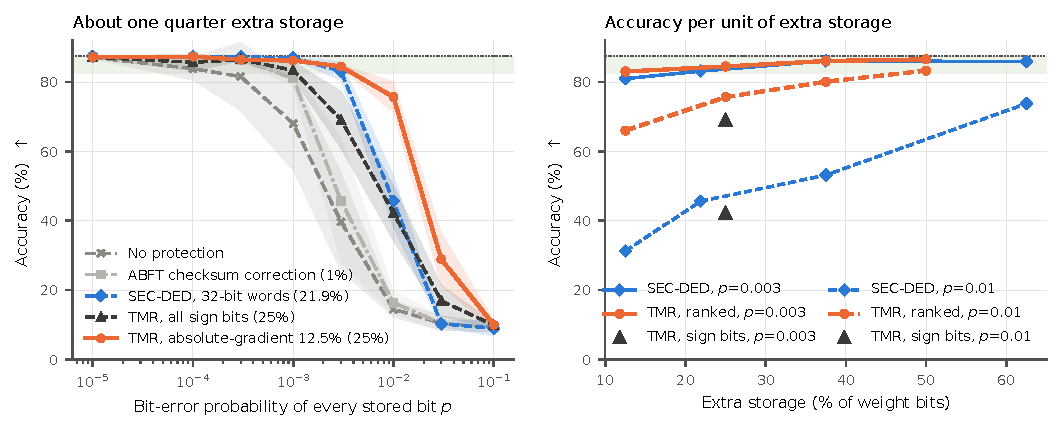
\includegraphics[width=\linewidth]{tecs_correction_mechanisms}
\caption{ResNet-8, protection mechanisms at equal extra storage. Every stored bit, including copies and check bits, flips with probability $p$. Bands are 95\% intervals over eight fault draws; the shaded region is the usefulness margin. Left: schemes costing about a quarter of the weight storage. Right: accuracy against extra storage at $p=3\times10^{-3}$ (solid) and $10^{-2}$ (dashed). ABFT checksum correction stores two checksums per output channel ($\approx$1\%).}\label{fig:correction}
\Description{Accuracy against bit-error probability and against extra storage for TMR of ranked bits, SEC-DED codes, ABFT checksum correction and TMR of sign bits.}
\end{figure}

The outcome depends on the fault rate (Fig.~\ref{fig:correction}). Up to $p=10^{-3}$ the codes are slightly better, by 0.7 to 1.4 accuracy points; near $3\times10^{-3}$ the two are equivalent; from $10^{-2}$ on, triplicating ranked bits is far better. At $p=10^{-2}$ and 12.5\% extra storage it keeps 66.0\% accuracy against 31.3\% for SEC-DED over 64 bits, a paired difference of 34.7 points (interval 25.7 to 43.8); at 25\% it keeps 75.7\% against 45.6\% for SEC-DED over 32 bits (21.9\% storage) and 42.3\% for TMR of all sign bits. Against sign-bit TMR of equal cost the ranked mask is better at every BER from $10^{-3}$ on, by 15.4 points (7.1 to 23.6) at $3\times10^{-3}$. ABFT checksum correction recovers almost nothing above $10^{-3}$, because almost every output channel then holds two or more faulty weights. Codes fail when two errors land in one word, which becomes likely at dense fault rates, while TMR of a bit fails only when two of its own three copies flip. By the usefulness criterion the gain is smaller: at 25\% and 37.5\% storage both ranked TMR and the code stop at $3\times10^{-3}$. The comparison counts storage only; voters, encoders, decoders, interleaving and scrubbing are not modelled, and it covers one checkpoint and one input window.


\Branch{R3a}{A bit-level simulation of each mechanism matches its residual curve in Table~\ref{tab:mechanisms} at every rate \TBD{}, including the wrong-repair rate of the checksum decoder.}{\TBD{which curves departed from simulation}.} The curves explain the ordering above: codes keep a $p^2$ law only while a second error in a word is unlikely, near $p<1/n$, and checksum correction over channels of hundreds of weights leaves it already near $p\approx10^{-4}$ (Fig.~\ref{fig:residual}). \Branch{R3b}{Letting the rate-aware assignment choose between three and five copies per bit improves on ranked triplication by \TBD{} at equal storage.}{Choosing between three and five copies per bit did not improve on ranked triplication \TBD{}.}
